%!TeX root = ../My_thesis.tex


% @inproceedings{my-dataset,
%     title = "Crowdsourced Corpus of Sentence Simplification with Core Vocabulary",
%     author = "Katsuta, Akihiro  and
%       Yamamoto, Kazuhide",
%     booktitle = "Proceedings of the Eleventh International Conference on Language Resources and Evaluation ({LREC} 2018)",
%     month = may,
%     year = "2018",
%     address = "Miyazaki, Japan",
%     publisher = "European Language Resources Association (ELRA)",
%     url = "https://www.aclweb.org/anthology/L18-1072",
% }


% .---|||___|||--- C H A P T E R ---|||___|||---. %
\chapter{Детали практической реализации}
% .---|||___|||--- C H A P T E R ---|||___|||---. %


% .---|||___|||--- S E C T I O N ---|||___|||---. %
\section{Выбор инструментов}
% .---|||___|||--- S E C T I O N ---|||___|||---. %


В данной работе используются следующие инструменты:
\begin{enumerate}[1.]%
  \item Машинное обучение. Для обучения модели будет использоваться Python в связке с фреймворком для машинного обучения PyTorch~\cite{PyTorch}, предоставляющий широкие возможности для реализации нейронных сетей, в том числе, там присутствует поддержка ранее упомянутых Transformer'ов.
  \item Токенизация. Для токенизации японского текста будет использоваться библиотека MeCab~\cite{MeCab}.
  \item Эмбеддинги. Готовые модели с эмбеддингами могут быть взяты из Python-библиотеки FastText~\cite{FastText} (в том числе там есть эмбеддинги для японского языка).
  \item Сервер. Тут, опять же, будет использован Python с фреймворком Falcon~\cite{Falcon}, позволяющим создавать легковесный back-end. То есть будет реализован REST API сервер.
  \item Веб-приложение. Будет использоваться TypeScript~\cite{TypeScript} с библиотекой Lit~\cite{Lit} (библиотека для веб-компонентов).
\end{enumerate}

Система будет доступна в браузере в виде простого веб-приложения, то есть модель будет обучена на Python, а пользоваться обученной моделью можно будет в любом современном браузере (пользователю ничего не нужно будет устанавливать).


% .---|||___|||--- S E C T I O N ---|||___|||---. %
\section{Как устроен Transformer изнутри}
% .---|||___|||--- S E C T I O N ---|||___|||---. %


Для ускорения вычислений в PyTorch используются не матрицы размерности~$N \times M$, а тензоры размерности~$B \times M \times N$ (где $B$ "--- размер батча), то есть матрицы обрабатываются батчами размера~$B$. Ускорение происходит за счёт оптимизированного вычисления батчей на видеокартах в PyTorch. Однако для простоты изложения будем считать, что работаем мы с матрицами.


% .---|||___|||--- S U B S E C T I O N ---|||___|||---. %
\subsection{Механизм внимания}
% .---|||___|||--- S U B S E C T I O N ---|||___|||---. %


Вернёмся к формуле~\eqref{scaled-dot-product-attention}. Программно её можно реализовать следующим образом:

\begin{minted}[tabsize=2, mathescape, linenos, xleftmargin=20pt, fontsize=\scriptsize]{python}
def scaledDotProductAttention(
  query: Tensor,
  key: Tensor,
  value: Tensor,
  mask: Optional[Tensor] = None
) -> Tensor:
  # Считаем scale, на который будем делить
  scale = query.size(-1) ** 0.5
  # Перемножаем матрицы query и key, делим их на scale
  temp = query.bmm(key.transpose(1, 2)) / scale

  # Применяем маску, если она есть
  if (mask is not None):
    temp += mask

  # Применяем softmax к измерению embedding'ов
  softmax = f.softmax(temp, dim=-1)
  # Перемножаем softmax с матрицей value
  return softmax.bmm(value)
\end{minted}

Обратим внимание на то, что в коде используется некая маска. О том, что это и зачем она нужна, поговорим в следующем разделе.


% .---|||___|||--- S U B S E C T I O N ---|||___|||---. %
\subsection{Маска в механизме внимания}
% .---|||___|||--- S U B S E C T I O N ---|||___|||---. %


Как же выглядит маска? Просто создаётся треугольная матрица формы $ \text{size} \times \text{size} $, в левой части которой «$0$», а в правой "--- «$-\infty$». Нужно это для того, чтобы при обучении не показывать полностью переведённые (упрощённые) предложения модели (защита от переобучения). То есть «$-\infty$» при суммировании маски со scores заставляет модель «принебречь» частями предложения. Вид матрицы представлен на~\firef{mask-matrix}.

\begin{equation}\label{mask-matrix}%
  \begin{bmatrix}
    0 & -\infty & -\infty & -\infty \\
    0 & 0 & -\infty & -\infty \\ 
    0 & 0 & 0 & -\infty \\ 
    0 & 0 & 0 & 0 \\ 
  \end{bmatrix}  
\end{equation}

Реализовать создание такой матрицы довольно несложно, в PyTorch это можно сделать следующим образом:

\begin{minted}[tabsize=2, mathescape, linenos, xleftmargin=20pt, fontsize=\scriptsize]{python}
def generateSquareSubsequentMask(size: int, device: torch.device) -> Tensor:
  # Создаём треугольную матрицу
  mask = (torch.triu(torch.ones((size, size), device=device)) == 1).transpose(0, 1)
  # Переводим её в формат float с 0-ми и -inf
  mask = mask.float() \
    .masked_fill(mask == 0, float("-inf")) \
    .masked_fill(mask == 1, float(0.))
  return mask
\end{minted}


% .---|||___|||--- S U B S E C T I O N ---|||___|||---. %
\subsection{Positional Encoding}
% .---|||___|||--- S U B S E C T I O N ---|||___|||---. %


Реализовать positional encoding тоже не составляет большого труда:

\begin{minted}[tabsize=2, mathescape, linenos, xleftmargin=20pt, fontsize=\scriptsize]{python}
def positionalEncoding(
  sequenceLength: int,
  dModel: int,
  device: torch.device
) -> Tensor:
  # Тензор [[[0.], [1.], [2.], ...]]
  pos = torch \
    .arange(sequenceLength, dtype=torch.float, device=device) \
    .reshape(1, -1, 1)
  # Тензор [[[0., 1., 2., ...]]]
  dim = torch.arange(dModel, dtype=torch.float, device=device).reshape(1, 1, -1)
  # Фаза (аргумент для cos/sin) =
  # [
  #   [
  #     [0., 0., 0., ...],
  #     [1., 1., 1., ...],
  #     [2., 2., 2., ...],
  #     ...
  #   ]
  # ]
  phase = pos / 10000 ** (dim // dModel)

  # [[[sin(...),  cos(...), sin(...),  cos(...), ...], ...]]
  return torch.where(dim.long() % 2 == 0, torch.sin(phase), torch.cos(phase))
\end{minted}


% .---|||___|||--- S U B S E C T I O N ---|||___|||---. %
\subsection{Как encoder учится понимать контекст}
% .---|||___|||--- S U B S E C T I O N ---|||___|||---. %


Чтобы научить encoder понимать смысл текста на каком-либо языке, нужно его каким-то образом обучить (предоставить данные для обучения).
Отличная новость заключается в том, что данные для обучения можно получить относительно несложно, причём в очень больших объёмах.
В модели BERT~\cite{BERTmodel}, к примеру, сделали следующее: для большого набора языков выгрузили все статьи википедии для каждого из них.
После этого процесс обучения заключается в том, чтобы передавать encoder'у предложения, но не в исходном виде, а с замаскированными словами (вспомним маску, о которой мы говорили ранее), чтобы encoder пытался угадать, какое слово должно стоять в предложении.
Тоже самое делается и с предложениями "--- модели подаются 2 предложения, и она должна определить, следует ли оно предложение за другим.
Вся прелесть в том, что весь этот процесс обучения не нуждается в ручной обработке "--- маскировка случайных слов и подставление двух случайных предложений реализуется программно, причём довольно просто.

После чего эти большие объёмы данных прогоняются через encoder, обучая его, а на выходе мы получаем модель, имеющую довольно обширное знание о законах языка, о том, как строятся слова в предложениях, а также как строятся сами предложения. Далее нужно лишь дообучить decoder для решения нужной нам задачи (fine-tuning), что можно сделать даже на относительно небольшом массиве данных. В итоге мы получаем модель, превосходящую современные решения в мире NLP.


% .---|||___|||--- S E C T I O N ---|||___|||---. %
\section{Сервер}
% .---|||___|||--- S E C T I O N ---|||___|||---. %


Как уже было сказано ранее, сервер использует фреймворк Falcon.
Имеется лишь один путь "--- \texttt{/processJapaneseText}, по которму пользовательское приложение передаёт запрос с японским текстом, после чего сервер, используя функции \texttt{parse}~и~\texttt{simplify}, упрощает это предложение и возвращает результат приложению.


% .---|||___|||--- S U B S E C T I O N ---|||___|||---. %
\subsection{Настройка сервера}
% .---|||___|||--- S U B S E C T I O N ---|||___|||---. %


Чтобы использовать сервер, его необходимо сначала настроить.
Так как написан он на Python, нам, естественно, понадобится установленный Python и менеджер пакетов pip, который поставляется вместе с ним.

Далее требуется установить необходимые зависимости через pip:
\begin{itemize}%
  \item \texttt{pip install falcon} "--- фреймворк Falcon,
  \item \texttt{pip install mecab} "--- библиотека MeCab,
  \item \texttt{pip install pytorch} "--- библиотека PyTorch,
  \item \texttt{pip install fasttext} "--- библиотека FastText,
  \item \texttt{pip install waitress} "--- библиотека для запуска сервера (для Windows),
  \item \texttt{pip install gunicorn} "--- библиотека для запуска сервера (для UNIX).
\end{itemize}

Теперь сервер может быть запущен командой:
\begin{itemize}%
  \item \texttt{waitress-serve -{}-port=8000 server:app} "--- на Windows,
  \item \texttt{gunicorn -{}-port=8000 server:app} "--- на UNIX.
\end{itemize}


% .---|||___|||--- S E C T I O N ---|||___|||---. %
\section{Пользовательское приложение}
% .---|||___|||--- S E C T I O N ---|||___|||---. %


Пользовательское приложение выглядит довольно минималистично "--- есть форма ввода предложения, после нажатия на кнопку «Simplify» или нажатия «Enter» отправляется запрос на сервер (по пути \texttt{/processJapaneseText}), после чего ответ отображается в виде, как на~\firef{app-screen}.

Есть также возможность посмотреть перевод предложений (исходного и упрощённого) "--- при нажатии на ссылку «translation» открывается страница Google Translate с выбранным предложением "--- это может использоваться как некая опорная линия упрощения (что смысл не потерялся).

Цвета в предложениях (исходном и упрощённом) на~\firef{app-screen} указывают на часть речи какого-либо токена (слова).

\begin{figure}[H]%
  \centering
  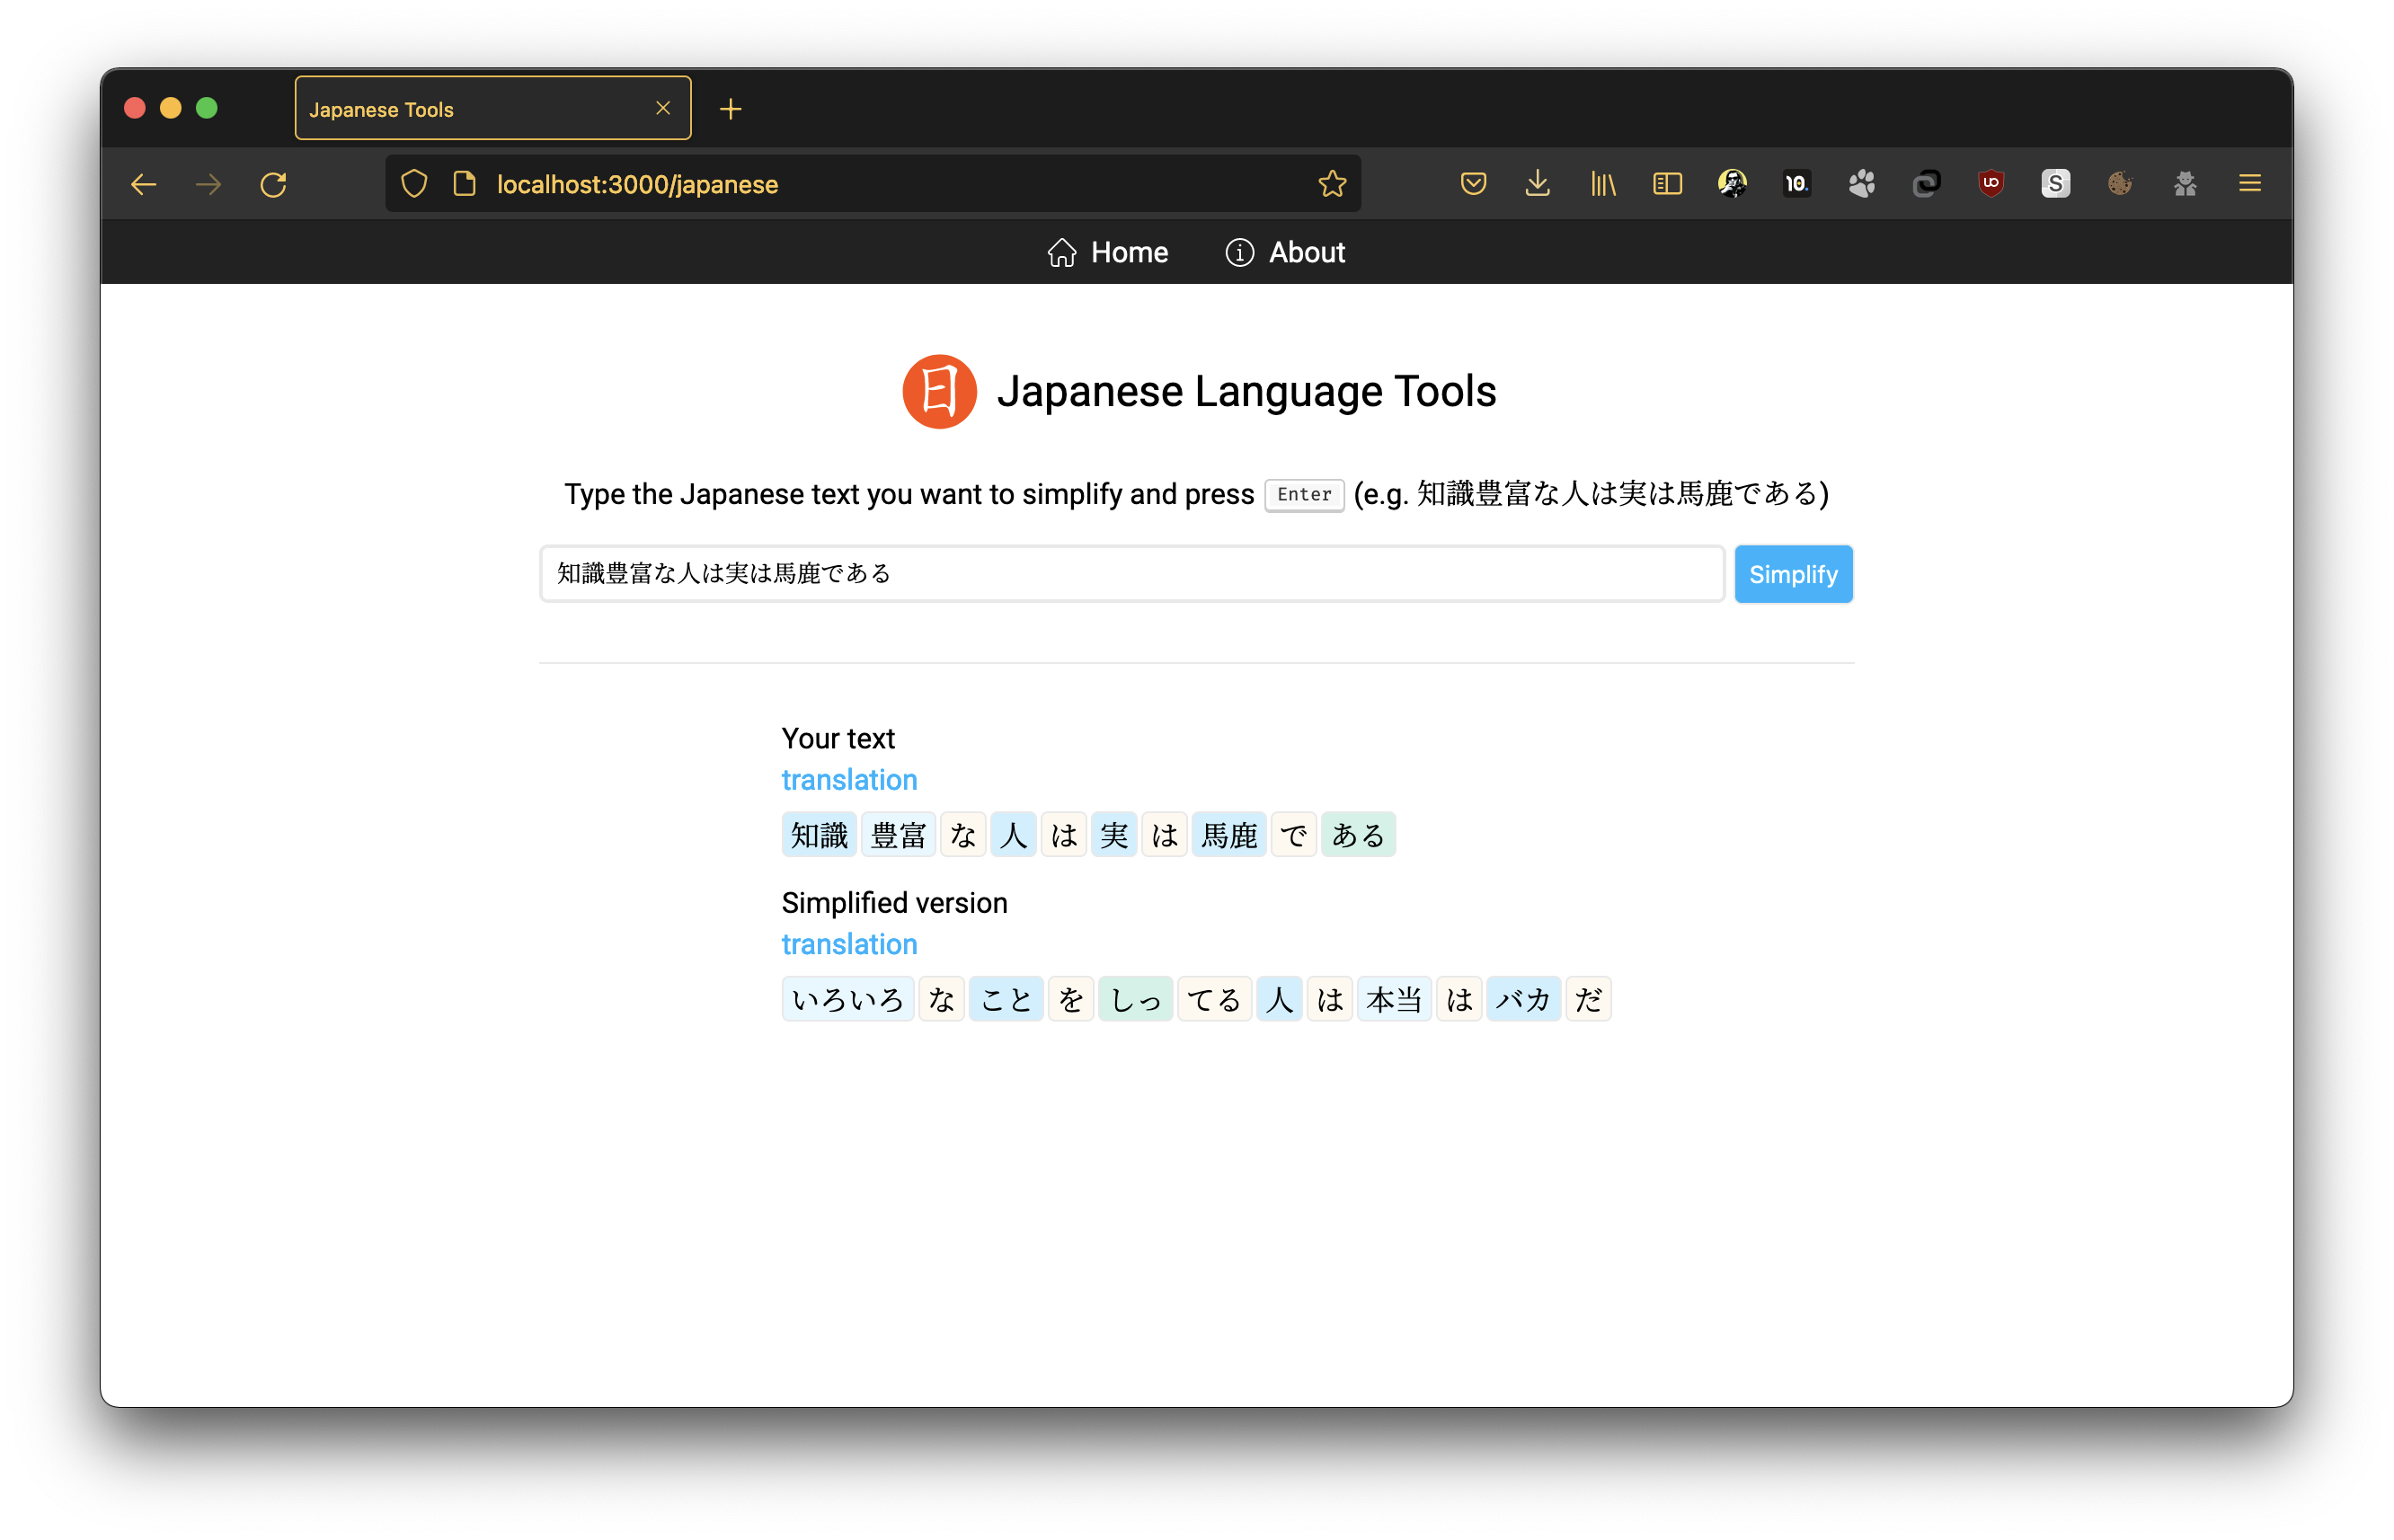
\includegraphics[width=\textwidth]{app.png}
  \caption{Пользовательское приложение}
  \label{app-screen}
\end{figure}


% .---|||___|||--- S E C T I O N ---|||___|||---. %
\section{Объяснение выбранной архитектуры}
% .---|||___|||--- S E C T I O N ---|||___|||---. %


Описанная архитектура «приложение-сервер» выбрана неслучайно. Дело в том, что в отличие, к примеру, от настольного приложения, пользователю ничего не нужно скачивать "--- он просто открывает веб-приложение и может пользоваться приложением. Обученная модель используется на сервере, что позволяет её чаще обновлять, а возможно даже и заменить на более удачную.

Это также может позволить другим разработчикам взять готовую часть решения "--- например, взять уже существующее приложение и использовать там свою модель для упрощения. Или же, наоборот, использовать в своём существующем приложении сервер, представленный в данной работе, просто делая к нему запрос по ранее упомянутому пути (так как сервер не имеет привязки к приложению, сделать это довольно просто, нужно лишь настроить домены, которым будет дан доступ к серверу).
